\documentclass[tikz, border=0.2cm]{standalone}

\usetikzlibrary{
	arrows, arrows.meta, positioning, decorations.markings, fit, 
	decorations.pathmorphing
}

\usepackage{amsmath, mathrsfs}

\begin{document}

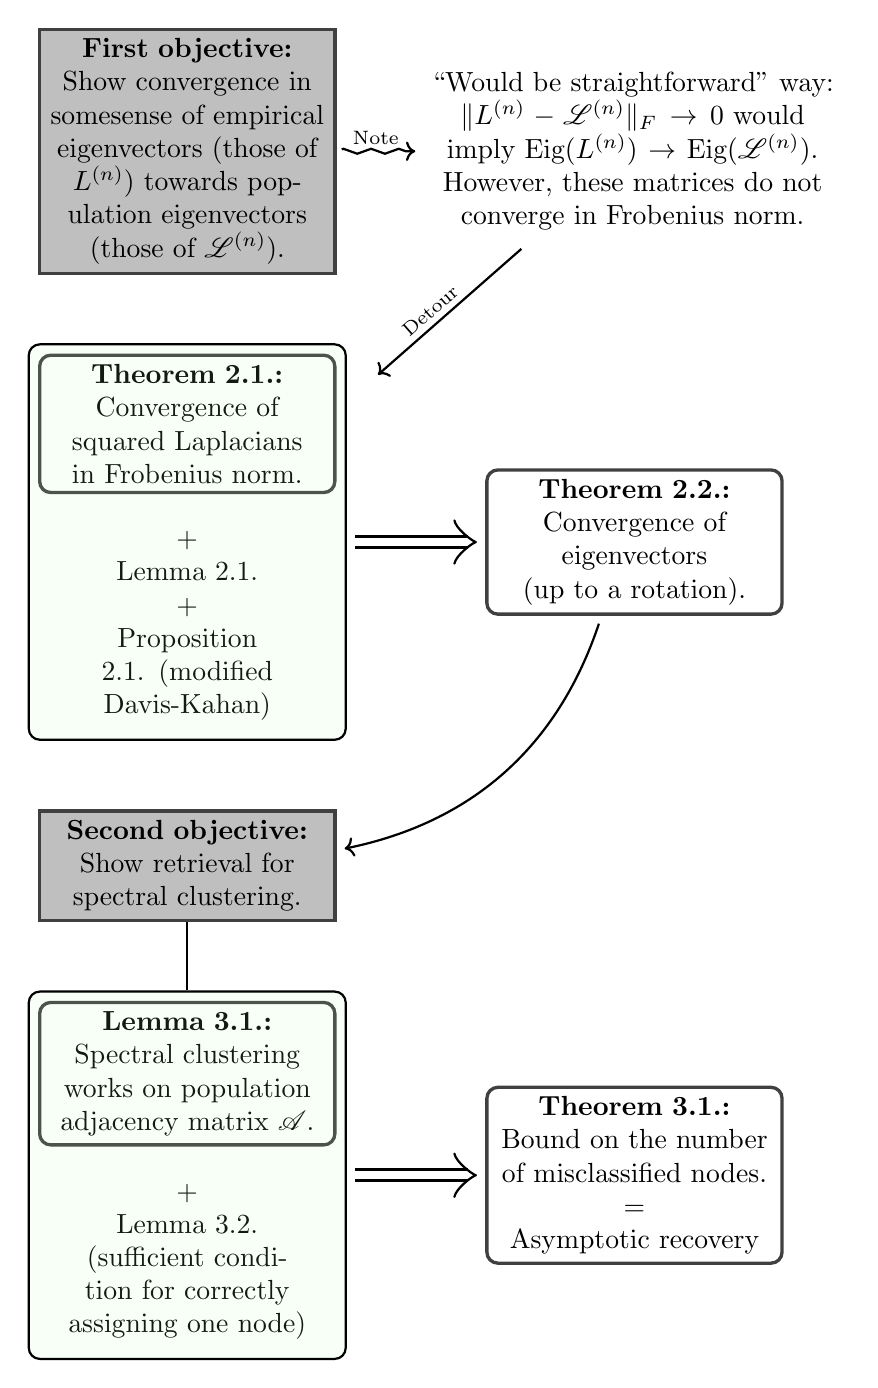
\begin{tikzpicture}[
	every node/.style={align=center, text width=10em},
	squarednode/.style={rectangle, draw=gray!50!black, fill=gray!50!white, 
		very thick, minimum size=7mm},
	roundnode/.style={rectangle, rounded corners, draw=gray!50!black, very 
		thick, minimum size=7mm}
	]
	
	% Nodes
	
	\node [squarednode] (1stobj) at (0,0) 
	{\textbf{First objective:}\\Show convergence in somesense of empirical 
		eigenvectors (those of \(L^{(n)}\)) towards population eigenvectors 
		(those 
		of \(\mathscr{L}^{(n)}\)).};
	
	\node [text width = 15em, align=center, right=of 1stobj] (straight) 
	{``Would be straightforward'' way:\\ \(\Vert L^{(n)} - 
		\mathscr{L}^{(n)} 
		\Vert_F \to 0\) would imply \(\text{Eig}(L^{(n)}) \to 
		\text{Eig}(\mathscr{L}^{(n)})\).\\However, these matrices do not 
		converge 
		in Frobenius norm.}; 
	
	\node [roundnode, below=of 1stobj] (thm21)
	{\textbf{Theorem 2.1.:}\\Convergence of squared Laplacians in Frobenius 
		norm.};
	
	\node [below=1em of thm21] (notesthm21) 
	{+\\Lemma 2.1.\\+\\ Proposition 2.1. (modified Davis-Kahan)};
	
	\node[
	roundnode,
	draw=black, thick, 
	fit=(thm21) (notesthm21), 
	fill=green!30!white, fill opacity=0.1] 
	(box1) {};
	
	\node [roundnode, right=5em of box1] (thm22)
	{\textbf{Theorem 2.2.:}\\Convergence of eigenvectors\\(up to a rotation).};
	
	\node[squarednode, below=of notesthm21] (2ndobj) 
	{\textbf{Second objective:}\\Show retrieval for spectral clustering.};
	
	\node[roundnode, below=of 2ndobj] (lemma31)
	{\textbf{Lemma 3.1.:}\\Spectral clustering works on population 
		adjacency matrix 
		\(\mathscr A\).};
	
	\node [below=1em of lemma31] (noteslemma31) 
	{+\\Lemma 3.2.\\(sufficient condition for correctly assigning one 
		node)};
	
	\node[
	roundnode,
	draw=black, thick, 
	fit=(lemma31) (noteslemma31), 
	fill=green!30!white, fill opacity=0.1] 
	(box2) {};
	
	\node [roundnode, right=5em of box2] (thm31) 
	{\textbf{Theorem 3.1.:}\\Bound on the number of misclassified 
		nodes.\\=\\Asymptotic recovery};
	
	% Arrows
	\path[->, shorten <= 2pt, thick, decoration={zigzag, amplitude=.9}] 
	(1stobj) 
	edge[decorate] 
	node[text width=2.5cm,midway, sloped, above=0.5em, anchor=center] 
	{\scriptsize Note}
	(straight);
	
	\path[->, shorten >= 15pt, shorten <= 5pt, thick]
	(straight)
	edge
	node[text width=2.5cm, midway, above=0.5em, sloped, anchor=center] 
	{\scriptsize Detour}
	(box1);
	
	\draw[
	line width=1pt, double distance=3pt,
	-{Classical TikZ Rightarrow[length=3mm]}, 
	shorten >= 3pt, shorten <= 3pt] 
	(box1) -- (thm22);
	
	\draw[
	line width=1pt, double distance=3pt,
	-{Classical TikZ Rightarrow[length=3mm]}, 
	shorten >= 3pt, shorten <= 3pt] 
	(box2) -- (thm31);
	
	\draw[thick] (2ndobj) -- (box2); 
	
	\path[thick, ->, shorten <= 3pt, shorten >= 3pt]
	(thm22) edge[bend left] (2ndobj);
	
\end{tikzpicture}

\end{document}
